%%%%%%%%%%%%%%%%%%%%%%%%%%%%%%%%%%%%%%%%%%%%%%%%%%%%%%%%%%%%%
%       		  Imperial College London
%   		      Department of Materials
%                MEng/MSc Thesis Template
%%%%%%%%%%%%%%%%%%%%%%%%%%%%%%%%%%%%%%%%%%%%%%%%%%%%%%%%%%%%%
%       Maintained by Jonathan Rackham and Andrew Cairns
%     j.rackham@imperial.ac.uk, a.cairns@imperial.ac.uk
%    Released under a Creative Commons CC BY 4.0 licence
%%%%%%%%%%%%%%%%%%%%%%%%%%%%%%%%%%%%%%%%%%%%%%%%%%%%%%%%%%%%%
% CHANGES
% v0.1  -copied in from Lit Review template
% v1.0  -change to report document class
%       -added ToC
%       -removed word count
%       -11pt font
%       -margins to 1.5cm, headsep to 0, headheight increased for clearance
%       -header set to section
%       -page number in footer
%       -add guidance from current thesis template
%
%
%
%%%%%%%%%%%%%%%%%%%%%%%%%%%%%%%%%%%%%%%%%%%%%%%%%%%%%%%%%%%%%
%describes the document we are making

%%%%%%%%%%%%%%%%%%%%%%%%%%%%%%%%%%%%%%%%%%%%%%%%%%%%%%%%%%%%%
%Document preamble, adds useful packages and sets up the document. 

\NeedsTeXFormat{LaTeX2e}
\documentclass[11pt,a4paper,twoside]{report}  %text size (11pt)


\usepackage{datetime}

\newcommand{\monthyeardate}{\ifcase \month \or January\or February\or March\or %
April\or May \or June\or July\or August\or September\or October\or November\or %
December\fi, \number \year} 
  

%----------------------------------------------------------------------------------------
%	FONTS AND TYPESETTING
%----------------------------------------------------------------------------------------
\usepackage[british]{babel}							%makes latex aware of your language, so better hyphenating etc
\usepackage[T1]{fontenc} 							%use the T1 for proper searching and use of ligatures etc
%\usepackage{microtype}								%enables microtypesetting, just makes things pretty
\usepackage{blindtext}                              %produces random text to fill space, useful to demonstrate things
\usepackage{csquotes}
\usepackage{xpatch}
\usepackage{fontspec} % Required for specifying custom fonts

\defaultfontfeatures{Ligatures=TeX} % To support LaTeX ligatures (e.g. `` and --)
\defaultfontfeatures{Path=Fonts/} % Specify the location of font files

% The default font family
\setmainfont{ImperialSansText}[
	UprightFont=*-Regular.ttf,
	%BoldFont=*-Bold.ttf
        BoldFont=*-Semibold.ttf
]

% The monospace font used explicitly with \texttt{}/\ttfamily
\setmonofont{ImperialSansText}[
	UprightFont=*-Regular.ttf,
	%BoldFont=*-Bold.ttf
        BoldFont=*-Semibold.ttf
]

\newfontfamily{\ImperialSansMedium}{ImperialSansText}[
	UprightFont=*-Medium.ttf,
	BoldFont=*-Semibold.ttf,
]

% Define the other Imperial Sans font weights
\newfontface{\ImperialSansExtraBold}{ImperialSansText-Extrabold.ttf}
\newfontface{\ImperialSansExtraLight}{ImperialSansText-Extralight.ttf}
\newfontface{\ImperialSansSemiBold}{ImperialSansText-Semibold.ttf}
\newfontface{\ImperialSansLight}{ImperialSansText-Light.ttf}



%----------------------------------------------------------------------------------------
%	COLORS
%----------------------------------------------------------------------------------------

% Convert colors to CMYK space if the print class option was used
%\iftoggle{print}{
%	\usepackage[svgnames, cmyk]{xcolor} % Required for defining and using custom colors
%{
	\usepackage[svgnames]{xcolor} % Required for defining and using custom colors
%}

\definecolor{ICLBlue}{RGB}{0, 0, 205}






%----------------------------------------------------------------------------------------
%	PAGE LAYOUT
%----------------------------------------------------------------------------------------
\usepackage[singlespacing]{setspace}				%adjusts linespacing, you may want to use onehalfspacing for drafts
\usepackage{geometry}				                %adjusts page layout including margins
\geometry{margin=1.5cm,headheight=16pt,headsep=3mm}	%the page geometry as defined, A4=210x297mm
\pagestyle{plain}						            %includes page number in centred in footer
\usepackage{fancyhdr}
\pagestyle{fancy}
\fancyhead{} 									%clears all header fields
\fancyhead[R]{\leftmark} 						% gives the level 1 sectioning title (\leftmark) on the RHS of header
\fancyfoot{} 									%clears all footer fields
\fancyfoot[L]{\ImperialSansSemiBold{Imperial College London}} 					%Imperial in footer
\fancyfoot[C]{\thepage} 					%page number in centre of footer

%%%% REMEMBER TO UPDATE!%%%
\fancyfoot[R]{YI FANG TOO} 					%Your Name
%%%% REMEMBER TO UPDATE!%%%


\usepackage{emptypage}								%if a page is empty then no header and foot are printed
\setcounter{secnumdepth}{1}                     %limit section numbering to sections and subsections.
\setcounter{tocdepth}{1}                        %ToC shows sections and subsections.


%----------------------------------------------------------------------------------------
%	MATHS
%----------------------------------------------------------------------------------------
\usepackage{mathtools} 								%for the rendering of maths
\numberwithin{equation}{section}					%reset numbering within a structural object
\numberwithin{figure}{section}						%reset numbering within a structural object


%----------------------------------------------------------------------------------------
%	SCIENCE
%----------------------------------------------------------------------------------------
\usepackage[version=4]{mhchem}						%typesetting of chemical formulae
\usepackage{siunitx}								%typesetting of units and quantities with uncertainties etc, see the next few lines for options that have been set
\sisetup{detect-all, detect-weight=true, detect-family=true}  %  if the rest of the text is bold the units will be as well
\sisetup{range-units=single}  						% don't include units in both parts of an \SIrange ie 30-40 ppm not 30 ppm - 40 ppm.
\sisetup{multi-part-units=single}					% don't repeat units for multi-part numbers such as numbers with uncertainties. As above, but for quantities with uncertainties 
\sisetup{separate-uncertainty}						%list values with uncertanties as X\pm Y rather than X(Y).


%----------------------------------------------------------------------------------------
%	FIGURES AND TABLES
%----------------------------------------------------------------------------------------
\usepackage{caption}                                %enables captions for floats (ie figures and tables), see 
\usepackage{graphicx}								%for the rendering of floating graphics
\usepackage[section]{placeins}						%defines float barriers at the end of sections, so all figures must be placed before a new section can begin.
\usepackage{array} 								%for creating tables
\usepackage{booktabs}								%professional looking tables, provides /toprule etc
\usepackage{multirow}
\newcolumntype{R}[1]{>{\raggedleft\arraybackslash}p{#1}} % Define a new right-aligned paragraph column type
\newcolumntype{L}[1]{>{\raggedright\arraybackslash}p{#1}} % Define a new left-aligned (no justification) paragraph column type
\newcolumntype{C}[1]{>{\centering\arraybackslash}p{#1}} % Define a new centered paragraph column type

\setlength{\arrayrulewidth}{1pt} % Thickness of table rules


%----------------------------------------------------------------------------------------
%BIBLIOGRAPHY - UPDATE ME
%----------------------------------------------------------------------------------------
%This has been set up to use the referencing style of the journal Angewandte Chemie, identical in style to the journal Advanced Materials
% \usepackage{biblatex-chem}
\usepackage[style=chem-angew]{biblatex}

%----------------------
\DeclareCiteCommand{\supercite}[\mkbibsuperscript]      %put square brackets around the superscript citation numerals.
  {\usebibmacro{cite:init}%
   \let\multicitedelim=\supercitedelim
   \iffieldundef{prenote}
     {}
     {\BibliographyWarning{Ignoring prenote argument}}%
   \iffieldundef{postnote}
     {}
     {\BibliographyWarning{Ignoring postnote argument}}%
  \bibopenbracket}%
  {\usebibmacro{citeindex}%
   \usebibmacro{cite:comp}}
  {}
  {\usebibmacro{cite:dump}\bibclosebracket}

%%%%%   CHANGE ME  %%%%%
\addbibresource{./references.bib}	%the absolute or relative path of your bibliography file.
%%%%%   CHANGE ME  %%%%%

%----------------------------------------------------------------------------------------
%	DOCUMENT NAVIGATION
%----------------------------------------------------------------------------------------
\usepackage{hyperref, bookmark}						%turns the references and citations into hyperlinks. This needs to be last on the preamble.
\hypersetup{colorlinks=true,linkcolor=black,citecolor=blue,urlcolor=blue}

\usepackage{comment}
\usepackage{xcolor}
\newcommand{\red}[1]{{\color{red}#1}}



%%%%%%%%%%%%%%%%%%%%%%%%%%%%%%%%%%%%%%%%%%%%%%%%%%%%%%%%%%%%%%%


\begin{document}
%	Put the document stuff in here!


\begin{titlepage}			%makes a title page. Remember to change the author, CID, username and to what is appropriate for you!

\begin{center}

\vspace{3cm}

\LARGE{{Department of Materials}}\\
\LARGE{{Imperial College London}} \\


\vspace{2cm}

\includegraphics[width=4cm]{img/Crest.png}

\vspace{2cm}

\LARGE{{MEng Project Report}\\
2025--6}

\vspace{1.6cm}

\Large{{Supervisors: Professor Johannes Lischner, Professor Ju Li, Assistant Professor Haowei Xu}}

\vspace{1.6cm}



	\color{ICLBlue} % Color
	\renewcommand\arraystretch{2.5} % Increase table row heights
	\setlength\extrarowheight{-2pt} % Vertically center the content of table cells
    %\setlength{\tabcolsep}{18pt}
	\begin{tabular}{@{} L{0.29\linewidth} @{} | @{\hspace{0.4cm}} L{0.6\linewidth} @{}}
		\hline % Top rule
		\Huge{Yi Fang Too} & \Huge{\ImperialSansSemiBold{Predicting Electronic Properties of Nanomaterials with Deep Learning Hamiltonians}}\\
        & \\
        &\\
          &\\
		\hline % Bottom rule
	\end{tabular}

\end{center}

\ImperialSansSemiBold{Imperial College London}
\end{titlepage}

\cleardoublepage 
\phantomsection


\begin{abstract}\label{sec:abstract}            %an abstract
    Here include an abstract summarising the thesis and its main results in less than 200 words (recommended: up to 150): what was done, what you found, and what is the significance of the results. It should appear before the table of contents.
    

\end{abstract}


\cleardoublepage

\pagenumbering{roman}
\tableofcontents


\section*{ }


\section*{AI declaration}    %the star here means the section is unnumbered and doesn't appear in the TOC
Describe your use of artificial intelligence (AI), including GenAI, in your thesis, in complete sentences. All other work is my own unless otherwise stated.  

\section*{Collaboration and supervision}    %the star here means the section is unnumbered and doesn't appear in the TOC


Briefly include a commentary on relationship to previous work e.g. in summer placements or UROPs, industrial involvement, collaboration e.g. with linked PhDs and PDRA work. This is in order that the examiners have an appreciation for the context of the work and can distinguish which work is your, versus that included for context from previous or ongoing work.

Optical calculations for shift current conductivity were adapted from the work of Asst. Prof. Haowei Xu as detailed in the papers 

\section*{Acknowledgements}
Do thank other students, postdocs, your supervisor and all technical and administrative staff that helped you during your project here.

Thank you thank you thank you: Professor Johannes Lischner, Assistant Professor Haowei Xu, Professor Ju Li, Dr. Chengcheng Xiao, soon-to-be-Dr. Christopher Cheung, Professor Arash Mostofi (please please give me a decent mark), the Mostofi-Lischner group for invaluable presentation feedback, Aishah Faisal for being the goat, Professor Robin Grimes for also being the goat and not as scary as I expected

Special shoutout: StackOverflow I love You 

P/S to besties: 

\cleardoublepage      %start a new page
\pagenumbering{arabic}

\chapter{Aims and Context}

\section{Aims}

In this project, we set out to investigate the electronic properties of nanomaterials with deep-learning Hamiltonians. DeepH-E3, developed by Gong et. al., is a  neural network capable of predicting electronic Hamiltonians from a given set of input atomic coordinates and corresponding elements\autocite{gongGeneralFrameworkE3equivariant2023}. While it has been tested on large supercells and certain twisted bilayer systems, its performance on structures such as strained monolayers and narrow-walled nanotubes has not been explored. In this work, the applicability of this deep-learning model to complex unseen geometries was investigated, as well as methods for improvement. Systems studied include vacancies, nanotubes, and homogeneous strain. Three sets of training data were utilized: monolayer \ce{MoS2}, bilayer \ce{MoS2}, and monolayer graphene. 

\section{Context}

Nanomaterials, defined as materials with at least one dimension measuring between 1-100\,nm, have been the subject of significant interest and research since the discovery that they exhibit novel properties distinct from their bulk counterparts\autocite{liNanostructuredMaterialsPhysicochemical2023}. A pivotal moment in the field was the successful isolation of graphene, which displays ballistic electron transport, giant magnetoresistance, and strong current amplitudes\autocites{novoselovElectricFieldEffect2004, xinGiantMagnetoresistanceDirac2023}. Since then, two-dimensional (2D) materials such as graphene and transition metal dichalcogenides (TMDs) have enjoyed a high degree of attention, with proposed applications ranging from next-generation transistors to ultrashort pulsed lasers\autocites{novoselovElectricFieldEffect2004, zhangOpticalLimitingCarboxyl2017}. TMDs, a group of compounds with the chemical formula \ce{MX2} (M being a transition metal atom and X a chalcogen atom), are particularly sought after for optoelectronic applications as they possess direct bandgaps in their monolayer form\autocite{makAtomicallyThin$mathrmMoS_2$2010}.

Further enhancing the appeal of 2D materials is their versatility. A single sheet can be `rolled' to obtain one-dimensional nanotubes, `sliced' to give nanoribbons, wrinkled, bent, and more. Each of these configurations has been experimentally realised and shown to display distinct electronic effects. Graphene nanoribbons with a zigzag edge, for example, possess almost-flat bands at the Fermi level, while carbon nanotubes predate graphene in their discovery and have exceedingly high theoretical current densities in metallic form\autocites{nakadaEdgeStateGraphene1996,hongFlexibleApproachMobility2007}. Defects and strain can alter electronic properties significantly, in addition to being highly relevant to practical applications\autocites{changOrbitalAnalysisElectronic2013, joEffectsStrainDefects2024}. Last but not least, twisted bilayer materials can exhibit fascinating phenomena, a prominent example being unconventional superconductivity exhibited by bilayer graphene at a twist angle of 1.1$^\circ$ \autocite{caoUnconventionalSuperconductivityMagicangle2018}.

In order to fully utilise these nanomaterials, it is essential to accurately predict their behaviour. Electronic structure methods, which aim to simulate materials from first principles by solving the Schr\"{o}dinger equation, vary widely in their accuracy and computational cost. The current method of choice for electronic structure is density-functional theory (DFT), which takes advantage of the Hohenberg-Kohn theorem to predict the ground-state electronic density and energy instead of calculating the full ground-state wavefunction\autocite{hohenbergInhomogeneousElectronGas1964}. However, DFT is extremely time-consuming for large systems. For example, a calculation on magic-angle twisted bilayer graphene (with 11,164 atoms) occupied 5000 CPU cores for a month\autocite{lucignanoCrucialRoleAtomic2019}. 

In recent years, machine-learning (ML) has leapt to the forefront of materials simulation. ML centres around the usage of algorithms that improve with data to perform tasks such as classification or regression, and has found numerous applications in materials science\autocite{ruppGuestEditorialSpecial2018}. ML Hamiltonians--part of an emerging field at the intersection of ML and traditional physics-based simulation methods--aim to model the electronic Hamiltonian as function of atomic structure, typically utilising DFT data for training.

One such ML Hamiltonian is DeepH-E3. DeepH-E3, developed by Gong et. al. in 2022, learns from DFT data calculated for relatively small systems and is capable of generalising to supercells exceeding 1000 atoms with sub-meV accuracy at a fraction of the computational cost required by similar DFT calculations\autocite{gongGeneralFrameworkE3equivariant2023}. As such, it is highly promising for studies of large systems such as twisted bilayer materials, multi-walled nanotubes, defects, and so on.

\begin{comment}
Due to their reduced size and high surface-area-to-volume ratio, nanomaterials tend to possess increased specific strength, conductivity, catalytic properties, and enhanced optical effects. On top of these, their reduced dimensionality is highly desirable for downscaling of electronics, the ever present transistor grail.

Two-dimensional (2D) nanomaterials consist of an atomically thin layer. 2D materials can be single-layered, such as hexagonal boron nitride and graphene, or they can be tri-layered, such as transition metal dichalcogenides. The latter, consisting of a single layer of transition metal atoms sandwiched between two layers of chalcogen atoms (e.g. S, Se) with the chemical formula \ce{MX2}, have attracted attention in the last decade as potential . 


Nonlinear optical effects, which are higher-order responses to an applied optical field, have found various applications in fields ranging from photovoltaics to \cite{xuPureSpinPhotocurrent2021}. Low-dimensional materials are of particular interest due to their exotic behaviour, especially when layered\cite{yangSecondharmonicGeneration2D2024, abbasiLowDimensionalMaterialsNonlinear2025}. However, simulation of supercells is notoriously expensive when using DFT. In recent years, deep-learning Hamiltonians have emerged as a \cite{liDeeplearningDensityFunctional2022, gongGeneralFrameworkE3equivariant2023, liDeepLearningDensityFunctional2024}. 


The use of deep-learning Hamiltonians could potentially accelerate the evaluation of nonlinear optical properties and responses, especially for large-scale systems of interest such as twisted bilayer materials which have unique advantages in the field of nonlinear optics\cite{abbasiLowDimensionalMaterialsNonlinear2025}. 
\end{comment}



\section{Applications}

In order to meet sustainable development goals, as well as keep up with ever-increasing demands for faster and better technology, new materials which enable energy-efficient, lightweight devices are essential. Nanomaterials are perfectly suited to this purpose; by virtue of their size, they naturally enable shrinking technologies. Moreover, they tend to possess increased specific strength, conductivity, catalytic properties, and enhanced optical effects, rendering them suitable for applications in myriad fields from medicine to agriculture. 

\red{((more discussion about 2D materials specifically--in-plane quantum confinement -> FET applications; twistronics and topological insulators?))

((\ce{MoS2}, a transition-metal dichalcogenide, is among the most heavily-researched 2D materials.))}


\subsection{Technology}

\red{((Nanoelectronic devices, role of strain and defect engineering, importance of doping in electronic properties))}

\subsection{Energy and the environment}

\red{((Photovoltaics (thin film), solar cells, energy-efficient electronics, photocatalytic applications--nanoparticles also difficult to simulate))}



\chapter{Literature Review}

\section{Introduction}

The ability to accurately and efficiently predict the Hamiltonian of a complex system is invaluable. From the Hamiltonian, a variety of properties--including but not limited to the Berry phase, complex dielectric constant, and charge density--can be determined\autocite{liDeeplearningDensityFunctional2022}. By circumventing the barrier of long calculation times, deep learning Hamiltonians enable the possibility of establishing a library of twisted bilayer materials or systems with various defects, which can then be screened for desirable properties such as high-temperature superconductivity. In combination with machine-learning interatomic potentials, a relatively developed field which has already displayed promising results for nanomaterials, the entire pipeline of relaxing complex geometries such as twisted bilayer systems to their equilibrium configurations then calculating their electronic and optical properties might be simplified and accelerated to an enormous degree\autocite{liCriticalReviewMachine2025}. 

\red{(note: consistency between Moire and twisted bilayer)

((relation between atomic structure and functional properties))}

This literature review will begin by surveying the electronic and optical properties of nanomaterials, with an emphasis on \ce{MoS2}.  The physical origins of these properties will be detailed, alongside potential applications and research directions. This is followed by a discussion of electronic structure methods, particularly DFT. We then observe advances and challenges in machine learning pertinent to materials science. Various options for reproducing the electronic Hamiltonian via machine learning will be contrasted. Finally, we briefly discuss methods to obtain optical properties as a byproduct of electronic structure calculations, as well as future directions for deep learning Hamiltonians with respect to modelling nanomaterials. 



\section{Nanomaterials}

Nanomaterials vary widely in their overall size and dimensionality, from zero-dimensional quantum dots to three-dimensional nanoporous structures. However, this review will largely focus on two-dimensional and one-dimensional materials.

One of the key properties of nanomaterials resulting from their size is quantum confinement, whereby electrons are spatially restricted as the dimensions of the material approach their de Broglie wavelength, which is on the order of 100\,nm. This results in 

The 

\red{((Discussion of quantum wells, discretization of energy levels and recent applications--))}

\subsection{Properties of \ce{MoS2}}

\ce{MoS2}, a transition metal dichalcogenide, was selected for its high applicability to problems in fields ranging from this to that


\subsection{Geometries}

\subsubsection{Strained systems}

Strain engineering is among the simplest methods of tuning electronic structure\autocite{safiStrainTunableElectronic2022}. By modifying the , .

The most prominent effect of tensile strain is the shift from a direct to indirect bandgap. 

\subsubsection{Nanotubes}

\red{role as channels in electronic devices; less fragile than 2D sheets, mechanical properties, dependence of metallic/semiconducting behaviour of how they are rolled--importance of atomic structure}

\subsubsection{Defects}
Defects have long been a challenge to simulate with DFT due to the large number of atoms needed to accurately mimic realistic systems. \red{effect on properties--defect states, doping importance}


\section{Electronic-structure methods}

The core issue with solving the many-electron problem lies with the sheer size of the ground-state wavefunction, which scales exponentially with system size (to be exact, by a power of 3N where N is the number of electrons in the system). While numerical methods such as quantum Monte Carlo exist, they tend to be exceedingly demanding in terms of computational cost\autocite{foulkesQuantumMonteCarlo2001}. As a result, the majority of electronic structure methods today must simplify the many-electron wavefunction, whether by using an independent-electron approximation (such as the Hartree-Fock method); only considering near(est) neighbours (tight-binding methods); or by computing the ground-state electronic density rather than the wavefunction.

The latter is the realm of density-functional theory, by far the most popular electronic structure method today.


\subsection{Density-functional theory (DFT)}

DFT stands out due to its balance between predictive power and computational efficiency\autocite{marzariElectronicstructureMethodsMaterials2021}. Based on the Hohenberg-Kohn theorem, which states that the ground-state properties of a many-electron system can be obtained by minimizing a functional $E[\rho(\mathbf r)]$ of the electronic density $\rho(\mathbf r)$, modern DFT utilises an auxiliary system of one-electron orbitals defined to have the same density as the real system\autocite{hohenbergInhomogeneousElectronGas1964, kohnSelfConsistentEquationsIncluding1965}. The non-interacting electrons of this auxiliary system can then be solved self-consistently to find the real system's ground-state density and, from that, its properties. The energy of the system is defined as follows: -- change to one with $T_s[rho] and E_xc[rho]$

$$[-\frac{\hbar^2}{2m}\nabla^2+V(\vec r) +V_H(\vec r)+V_{XC}(\vec r)]\psi_i(\vec r)= \epsilon_i\psi_i(\vec r)$$

where $V_H$ is the Hartree potential and $V_{XC}$ is the exchange-correlation potential.


One especially attractive feature of DFT is its versatility and breadth of functionality. It is easily combined with other models to calculate multiple properties in a single computational run; for example, the majority of DFT programs offer the ability to obtain relaxed structures and interatomic forces using the Hellmann-Feynman theorem, or phonon dispersions via density-functional perturbation theory (DFPT). 

The advent of density-functional perturbation theory (DFPT)
\red{(discuss DFPT, TD-DFT, incorporation of spin)}

DFT is not without its disadvantages. The most glaring of these is visible in Equation \ref{equation:DFT}: its reliance on the XC functional, which is unknown and can only be approximated. 

\red{mention bandgap problem and how it is mitigated}

\red{approximations to XC functional-- LDA, GGA-PBE --recent advances in hybrid functionals-- meta-GGA, HSE== transition metal oxdides - standard oapproximations over-delocalise d-electrons (from perspective)}

\red{reproducibility}

The choice of basis set plays a key role in the accuracy of DFT calculations. 

Last but not least, the nature of the iterative self-consistent calculations--which involves repeatedly diagonalising the Hamiltonian--results in the computational cost of a calculation scaling cubically with the system size. While a vast improvement over the exponentially exploding ground-state wavefunction, this is enough to make one balk at simulating twisted bilayers, alloys, and other systems with upwards of a thousand atoms.


\subsection{Electronic structure methods for larger systems}

\subsubsection{Linear-scaling DFT}


Linear-scaling methods typically take one of two forms. The first form, orbital-free DFT, 
directly approximates the non-interacting kinetic energy $T_s[\rho]$, which in Kohn-Sham DFT is calculated exactly. Via bypassing the use of one-electron orbitals,  

The second approach utilises localised basis sets which exploit the locality of matter--i.e., beyond a certain cutoff radius, interatomic interactions become so negligible that they can be ignored. Unlike plane-wave basis sets, which are well-suited for periodic solids but extend over the , localised basis sets . Among the bases used for these . 

Linear-scaling codes such as ONETEP typically compute the DFT energy from the density matrix. The one-particle density matrix, $\rho(\mathbf r, \mathbf r') = \sum_{i} f_i\psi_i(\mathbf r)\psi^*_i(\mathbf r')$, serves as a starting point and provides a complete description of the Kohn-Sham system. Here $\{\psi_i\}$ are the orbitals and ...

ONETEP uses spatially localized orbitals expressed in terms of periodic sinc functions to ...

difference between this and stuff like openmx? role of the density matrix? does openmx use density matrix? recent developments?

Non-orthogonal basis sets 

\subsubsection{Tight-binding methods}


Since the states near the Fermi level are the most relevant, the full Hamiltonian does not always need to be calculated. Instead, a truncated Hamiltonian for states around the Fermi level can be approximated using a tight-binding matrix, whose elements represent the coupling strengths between sites. 

There are several methods of finding these coefficients. The simplest, empirical tight-binding, fits th

An alternative, \textit{ab initio} tight binding, utilises 

\red{methods of finding the hopping terms: wannier functions, empirical tight binding etc}


\section{Machine learning for materials}

In recent years, machine learning has emerged as a route to improve the efficiency of current methods by utilising models trained on experimental or computational results. This shift to data-driven approaches is partially driven by the wide availability of data via high-throughput DFT databases such as the Materials Project. 

\red{bit more background on ML--define some key terms like epoch, neural network, etc}

Efforts in this area are widespread and take many different approaches, ranging from learning quantum mechanical expectation values such as NMR shifts and atomic forces\autocite{ruppMachineLearningQuantum2015} to unsupervised learning of DFT wavefunctions using variational auto-encoders\autocite{houUnsupervisedRepresentationLearning2024}. As opposed to traditional physics-based approaches like DFT, ML has often been criticised for its 'black-box behaviour', ....

A major obstacle in the history of ML for materials was the representation of the crystal structure. Initial attempts involved augmenting the training data ........

A significant milestone in the field was the use of crystal-graph convolutional neural networks, ...

\red{discusss e3nns--used not just for hamiltonians; allegro, mace etc}

\red{areas and efforts: scaling, generalising --paragraph for advances in each e.g. physics-informed neural networks to improve performance}

\red{principles used: locality of basis, locality of matter, symmetry}

Research at the intersection of DFT and ML can be broadly divided into three categories: (1) the use of (2) machine-learning interatomic potentials (MLIPs) and (3) machine-learning Hamiltonians (ML Hamiltonians)\autocite{huangCentralRoleDensity2023}. 

MLIPs serve as an alternative to the empirical interatomic potentials used in molecular dynamics (MD). These attempt to recover the potential energy of a given system as a function of atomic positions, based on data from \textit{ab initio} MD trajectories\autocite{behlerPerspectiveMachineLearning2016}.

\subsection{ML Hamiltonians}

In contrast to MLIPs, ML Hamiltonians seek to recreate the Hamiltonian from a set of atomic positions. The electronic Hamiltonian has several key requirements which should ideally be met by its representation, namely: uniqueness; continuity; and invariance to translation, rotation and nuclear permutations\autocite{rupp_machine_2015}. The latter is particularly non-trivial.

\red{KRR, neural networks, etc}

One particular sub-field of ML which has been widely applied to ML Hamiltonians is deep learning. Deep learning . Each thingy is an epoch



Since the neural network is trained on DFT data, its accuracy is inherently limited. Nonetheless, one important advantage of machine learning methods for electronic structure is its speed: once a model has been trained--which could take anywhere from a matter of seconds to days, depending on the hyperparameters--it is capable of making predictions extremely quickly. \red{elaborate a bit...} 
It is also restricted by its basis set--in order to exploit the locality of electronic matter, the vast majority of ML Hamiltonians use a nonorthogonal localized orbital basis. While suitable for calculations on large systems, these have been shown to ....

\red{distinction between ML and deep learning--deep learning as subset, define neural network, brief overview of non-NN and their advantages/disadvantages}

Deep Hamiltonian neural networks (DHNNs) are trained on precomputed DFT Hamiltonian matrices and learn a direct mapping from atomic coordinates to the electronic Hamiltonian.

Besides advantages in efficiency, deep-learning Hamiltonians possess a unique advantage in the autodiff function, \red{DFPT, derivatives of response calculated analytically instead of finite diff method}

Another key shortcoming of machine learning Hamiltonians is their lack of transferability. (e.g. DeepH cannot be used for systems with atoms not in training set--related to basis) + scalability? 

Figure or table summarising types etc of neural networks and stuff

deeph precursors: phisnet (unke et al) = enn for hamiltonians of molecules with fixed system size + nigam et all with krr - rotationally equivariant features + zhang et al ACE hams of crystals


\red{key uses - noncollinear stuff, quantum transport, etc; EPC calculations are much much faster}

\red{challenges: spin-orbit coupling, topology?}

\red{taking positions only as input x completely describe system--dft can compute response to applied fields, deeph no}

\red{extension to time-dependence?}

\red{other approach where instead of learning from hamiltonian -- try to fit to get same output}

\section{Optical effects}



\section{Summary}



\chapter{Methods}

\section{Density-functional theory (DFT)}

The role of DFT in this project was two-fold. Firstly, it was used to generate training data for the neural network. Secondly, DFT calculations were carried out on the same structures evaluated by the neural network in order to verify its accuracy. Images of atomic structure and wavefunctions were obtained using OpenMX Viewer, a web-based molecular visualiser\autocite{leeOpenMXViewerWebbased2019}. 

\subsection{OpenMX\autocites{ozakiEfficientProjectorExpansion2005,ozakiNumericalAtomicBasis2004, ozakiVariationallyOptimizedAtomic2003, lejaeghereReproducibilityDensityFunctional2016}}

All DFT calculations were performed in OpenMX unless stated otherwise. OpenMX is an open-source DFT software utilizing numerically optimized pseudo-atomic basis functions; those used in this were generated by Ozaki et. al. using Adpack. DeepH-E3 is compatible with three DFT softwares, all based on molecular orbitals: OpenMX, SIESTA, and . Of the three, OpenMX was chosen as it had already been used in the publically available dataset. 

Optical conductivity and dielectric function tensors were also calculated with OpenMX. 

\subsubsection{Datasets}

Publically available datasets--also calculated using OpenMX--were used in training the monolayer graphene, monolayer \ce{MoS2}, and bilayer graphene models\autocite{gongDataset1GeneralFramework2023}. These were used in calculating the results published in the original paper for DeepH-E3, allowing for efficient benchmarking of model performance. 


\red{training data generation--use figure?}

Preparation of the . Firstly, AA and AB bilayers were created by hand with an arbitrary spacing. These were then relaxed to within () in order to determine the equilibrium interlayer spacing and atomic positions. The perturbation process was then applied. Firstly, .


All input files utilised in this project can be found on Zenodo at Ref \cite{}. 

\subsubsection{Complex geometries}

For the study of complex geometries, it was essential to obtain reference bandstructures. 

C2X was used to generate nanotubes, followed by a Python script to convert from .xyz to the desired OpenMX input file\autocite{rutterC2xToolVisualisation2018}.  

For the nanotubes, structural relaxations were carried out to within xxxx and relaxed only at the $\Gamma$-point. Nanotubes with < 180 atoms used an SCF k-grid of 1\,x\,1\,x\,8, whereas only the Gamma point was used for larger nanotubes. The Z-point in band calculations was set to the fractional coordinates (0.0, 0.0, 0.5).

defects etc: relaxation threshold and scf grid


\subsection{Quantum ESPRESSO\autocite{giannozziQUANTUMESPRESSOModular2009, giannozziAdvancedCapabilitiesMaterials2017}}
In addition to OpenMX, Quantum ESPRESSO was used to verify results and to obtain results of optical calculations not provided by OpenMX. Quantum ESPRESSO is an open-source plane-wave basis software. 

Norm-conserving pseudopotentials from the SG15 library were used in all Quantum ESPRESSO calculations\autocites{hamannOptimizedNormconservingVanderbilt2013, schlipfOptimizationAlgorithmGeneration2015}.

For the calculations of dielectric function, absorbance spectra, and joint density of states the \textit{epsilon.x} programme in QuantumESPRESSO was used. The formulae of each are detailed in the following section.


\section{DeepH-pack and DeepH-E3}

\autocites{liDeeplearningDensityFunctional2022,gongGeneralFrameworkE3equivariant2023}.

\subsection{Neural network architecture of DeepH-E3}

\subsection{The predicted Hamiltonian}

The original author suggests using inference tools from DeepH-pack to accelerate; hence, we used a combination of programs from DeepH-pack and DeepH-E3.

The Hamiltonian takes the following form:

In order to build the Hamiltonian in k-space, . The original inference utilises a simple Fourier transform. However, this resulted in issues when calculating the derivative of the Hamiltonian; ... replaced it with xxx. Insert equations from the code and stuff

Derivatives of the Hamiltonian are essential in predicting properties such as the transition dipole matrix strength and dielectric function. Due to the use of nonorthogonal localized orbitals as the basis set of DeepH-E3, the task of obtaining these derivatives is non-trivial; nonetheless, L\"{o}wdin orthogonalization can be utilised to transform the nonorthogonal Hamiltonian $\hat H^L(\vec k)$ into an orthogonal basis $\hat H^O(\vec k)$. More details can be found in ref. \cite{wangFirstprinciplesCalculationOptical2019}. 

\begin{align}
\hat H^O(\vec k) &= S^\frac12(\vec k) \hat H^L(\vec k)S^\frac12(\vec k) \\
\frac{\partial}{\partial k_i}\hat H^O(\vec k) &=  \\
\frac{\partial^2}{\partial k_i\partial k_j}\hat H^O(\vec k) &= 
\end{align}

\subsection{Training details}

\red{put in a table of the models trained, epochs trained for, data sources etc--maybe figure for train/val/test loss?}



\section{Electronic and optical properties}

The original DeepH-pack/DeepH-E3 models included an inferencing tool for the bandstructure calculated by diagonalizing the predicted Hamiltonian. The remaining properties included in this work were obtained using original code. 

In order to find the Fermi level, a bisection search is utilised after obtaining the density of states. A streamlined workflow is shown in Figure \ref{fig}. The number of electrons in the system is obtained from the OpenMX input file via an adapted preprocessing script. In semiconductors, the Fermi level is set to the middle of the gap. 

\red{DOS}

\begin{align}D(E) &= \int_{BZ} \frac{d^dk}{(2\pi)^d}\delta(E-E_k)\\ &= \frac1{N_k}\sum_{n,k}\delta(E-E_{n,k})\end{align}



where the Dirac-delta was approximated by a Gaussian with a smearing width of 5 meV: $$\delta(E-E_{n,k}) = \frac{1}{\sigma\sqrt{\pi}}\exp(-\frac{(E-E_{n,k})^2}{\sigma^2})$$.

\subsection{The momentum operator}

\red{working for momentum operator / dH/dk}

\begin{align}
\hat{H}_{\alpha,\beta}(\vec k) &= \langle \alpha \vec k|\hat H|\beta \vec k\rangle \\
&= \frac1N \sum_{\vec R,\vec R'}e^{i(\vec k\cdot (\vec R-\vec R')}\langle \alpha \vec R'|\hat H|\beta \vec R\rangle \\
\nabla_{\vec k}\hat H_{\alpha\beta} (\vec k) &= \frac1N \sum_{\vec R,\vec R'}i(\vec R-\vec R')e^{i(\vec k\cdot (\vec R-\vec R')}\langle \alpha \vec R'|\hat H|\beta \vec R\rangle\end{align}


 


Transition dipole matrix: $$\text{TDM}_i = |\langle\psi_{CBM}|\frac{\partial H}{\partial x_i}|\psi_{VBM}\rangle|^2$$


Nonlinear optical susceptibility was NOT calculated using the equation $$\chi^{ab} = \frac{e^2}{\varepsilon_0\hbar}\int \frac{d^3}{(2\pi)^3}\sum_{n,m} f_{nm}\frac{r^a_{nm}r^{b}_{mn}}{\omega_{mn}(k)-\omega-i\eta}$$ 


The fineness of the k-grid is an important parameter; as such, convergence studies were carried out for each calculation. The final k-grid was in .... size, taking .... seconds for a 3-atom system (monolayer \ce{MoS2}) and .... seconds for a 75-atom system (a $5\times 5$ \ce{MoS2} supercell).

JDOS: $$\frac1{N_k}\sum_{\vec k, m, n} \delta(E-(E_{m,\vec k}-E_{n,\vec k}))$$

Disregarding the intraband contribution, the equation used for the complex dielectric function was: $$\epsilon_{\alpha, \beta} = \delta_{\alpha\beta} +\frac{8}{N_k\Omega}\sum_{\vec k, m\neq n} \frac{\mathbf{M}_{\alpha, \beta}}{E_{m,k}-E_{n,k}}\frac{f(E_k,n)}{(\omega_{m,k}-\omega_{n,k})^2-\omega^2-i\Gamma \omega}$$ where $\mathbf{M}_{\alpha, \beta} = \langle$. \red{would like to discuss next meeting! still slightly off but looks promising?}

Atomic units, where  $\hbar=m_e=1$ and hence  $E = \hbar\omega=\omega$. As a result, the above equation simplifies to  $$\epsilon_{\alpha, \beta} = \delta_{\alpha\beta} +\frac{8}{N_k\Omega}\sum_{\vec k, m\neq n} \frac{\mathbf{M}_{\alpha, \beta}}{E_{m,k}-E_{n,k}}\frac{f(E_k,n)}{(E_{m,k}-E_{n,k})^2-E^2-i\Gamma E}$$


Additional check: integrate fermi factor over k, should =1

\section{Putting it all together: the workflow}

\begin{figure}[]      
	\centering				%put the figure in the middle of the page
	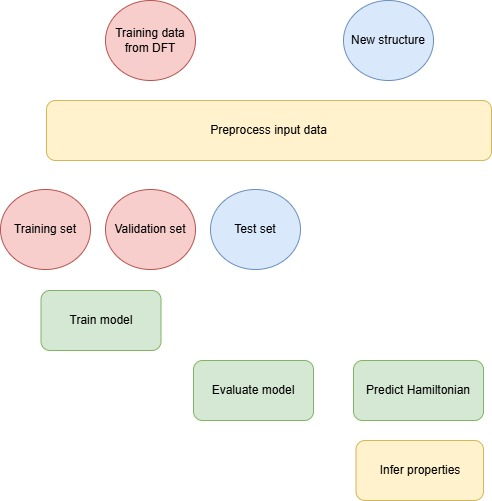
\includegraphics[height=15cm]{./img/methods workflow.jpg}			
	\caption{}		%Make your caption descriptive
	\label{fig:optical}			%so you can reference to the figure elsewhere using \ref{}
\end{figure}

\chapter{Results and Discussion}

\section{Monolayer \ce{MoS2}}

Firstly, we verified the performance of DeepH-E3 on monolayer \ce{MoS2}. \red{(2H, 1T, 1T')}


The RMSE calculated for the \ce{MoS2} bandstructure was as low as 0.088\,eV, which is highly promising. Divergences between DFT and DeepH do not appear until 20-30\,eV above the Fermi level, which is of negligible importance in most practical applications.

We also assessed its performance for randomly perturbed supercells. Three structures used in the original paper by Gong et al. were tested; the published results were successfully replicated. Three novel geometries where atoms were randomly perturbed with a vector of length between 0 and |0.3|\,\AA\ were also considered. 

\section{Homogenous strain}

Compressive and tensile homogenous strains ranging from 0\% to $\pm$10\% were applied by varying the size of the unit cell, then conducting a relaxation calculation on the atoms. \red{justify range chosen}

As seen in \ref{figure:strains}, the model performs with reasonable accuracy for strains below $\pm$5\%. Above $\pm$6\%, however, the results are unusable. 
The distribution of error throughout k-space is notably non-uniform, with strong valleys near the K-point and $\Gamma$-point for tensile and compressive strain respectively. \red{need to do more research on this part}

\red{Should I get some error bars in here? Perturb then strain or strain then perturb?}

The low tolerance for strain indicates that the training set had little variation in atomic positions. Connect to previous section with random supercells




\section{Nanotubes}

DeepH-E3 was also tested on nanotubes with radii ranging from 10\,\AA  to 50\,\AA. 

Figure \ref{figure} shows that the performance declines rapidly with decreasing nanotube radius. This is particularly troubling for multi-walled nanotubes, which contain too many atoms for DFT to handle with ease (i.e. without a GPU or significant time burden) but include a narrow nanotube which DeepH would surely struggle with. Similarly to the results for strain, the error rises drastically near the $\Gamma$ point, which could be a direct result of the . The magnitude of the error is compared to that of strain alone; approximate compressive and tensile strains are calculated with the following equations for tensile and compressive strain respectively: \begin{align}\varepsilon_{\text{tensile}} &= r_{\text{outer}}/r_{\text{middle}}\\\varepsilon_{\text{compressive}} &= r_{\text{inner}}/r_{\text{middle}}\end{align} 

\red{remark on whether curvature does/doesnt make a difference}

\section{Defects}

Defects exhibit characteristic energy levels within the bandgap, along with other variations in bandstructure. Both are dependent on the defect concentration and the type of defect. Since simulating interstitials and substitutional defects with atoms that are not Mo or S is not possible--a known limitation of DeepH-E3--we chose to look only at vacancies and substitutionals. 

\subsubsection{Vacancies}

Mo and S vacancies were simulated by removing an atom near the middle of a 5x5 supercell. The structures were then relaxed. Figure \ref{fig:vac} shows that DeepH is able to guess the presence of defect states in the bandgap, albeit not their position or quantity. Additionally, the shifts in the valence and conduction band are not accurately captured. 

\subsubsection{Substitutional defects}

\red{It would have been very cool to look at the wavefunctions but alas--my dreams may have to wait. Substitutionals should be fairly easy to do but I am spent at the moment. Will probably do on Tuesday}

\subsection{Improving performance for unseen geometries}

\red{To mimic the curvature of a nanotube while maintaining some similarity to the monolayer, 10x10 supercells were perturbed following a sine wave pattern, enabling periodic boundary conditions. The amplitude of the sine wave was randomly varied. The atoms were then, again, individually perturbed. To improve the behaviour for high strains, a larger variation in the magnitude was used, i.e. a normal distribution with a standard deviation of 0.15\,\AA. One atom was selected at random to be removed from the supercell, simulating a vacancy.}



\section{Bilayer \ce{MoS2}}

First, the monolayer-only model was tested on bilayer \ce{MoS2}. Since its performance was predictably abysmal, a separate model was trained on bilayer-only data. An attempt was made to use the monolayer model as a checkpoint and continue its training with the bilayer data, but its performance on the monolayer declined; as a result, it was concluded that continuing training with vastly different structures was not the best idea. We also looked at the performance of the monolayer for bilayer structures as a function of interlayer; since the electronic structure is mediated by the interlayer spacing, above 5\,\AA\ the DFT results display ??? and the bandstructures resemble those of a simple monolayer. As shown in \ref{fig:spacings}, 

The bilayer model was notably slower, which may have been due to the higher cutoff radius. As shown in \ref{fig:optical}, even after 4000 epochs, the MAE in both bandstructures and Hamiltonians was notably high. While bands near and below the Fermi level are captured accurately, the error associated with higher conduction bands is much less satisfactory.\red{(to note--the basis set doesn't include f orbitals at all--higher energy states bound to be problem? OpenMX calc was also spd only though)}

Randomly perturbed supercells, generated using the same process for the training data, were also used to assess its performance on unseen geometries. 

\section{Optical effects}

\begin{figure}[]      
	\centering				%put the figure in the middle of the page
	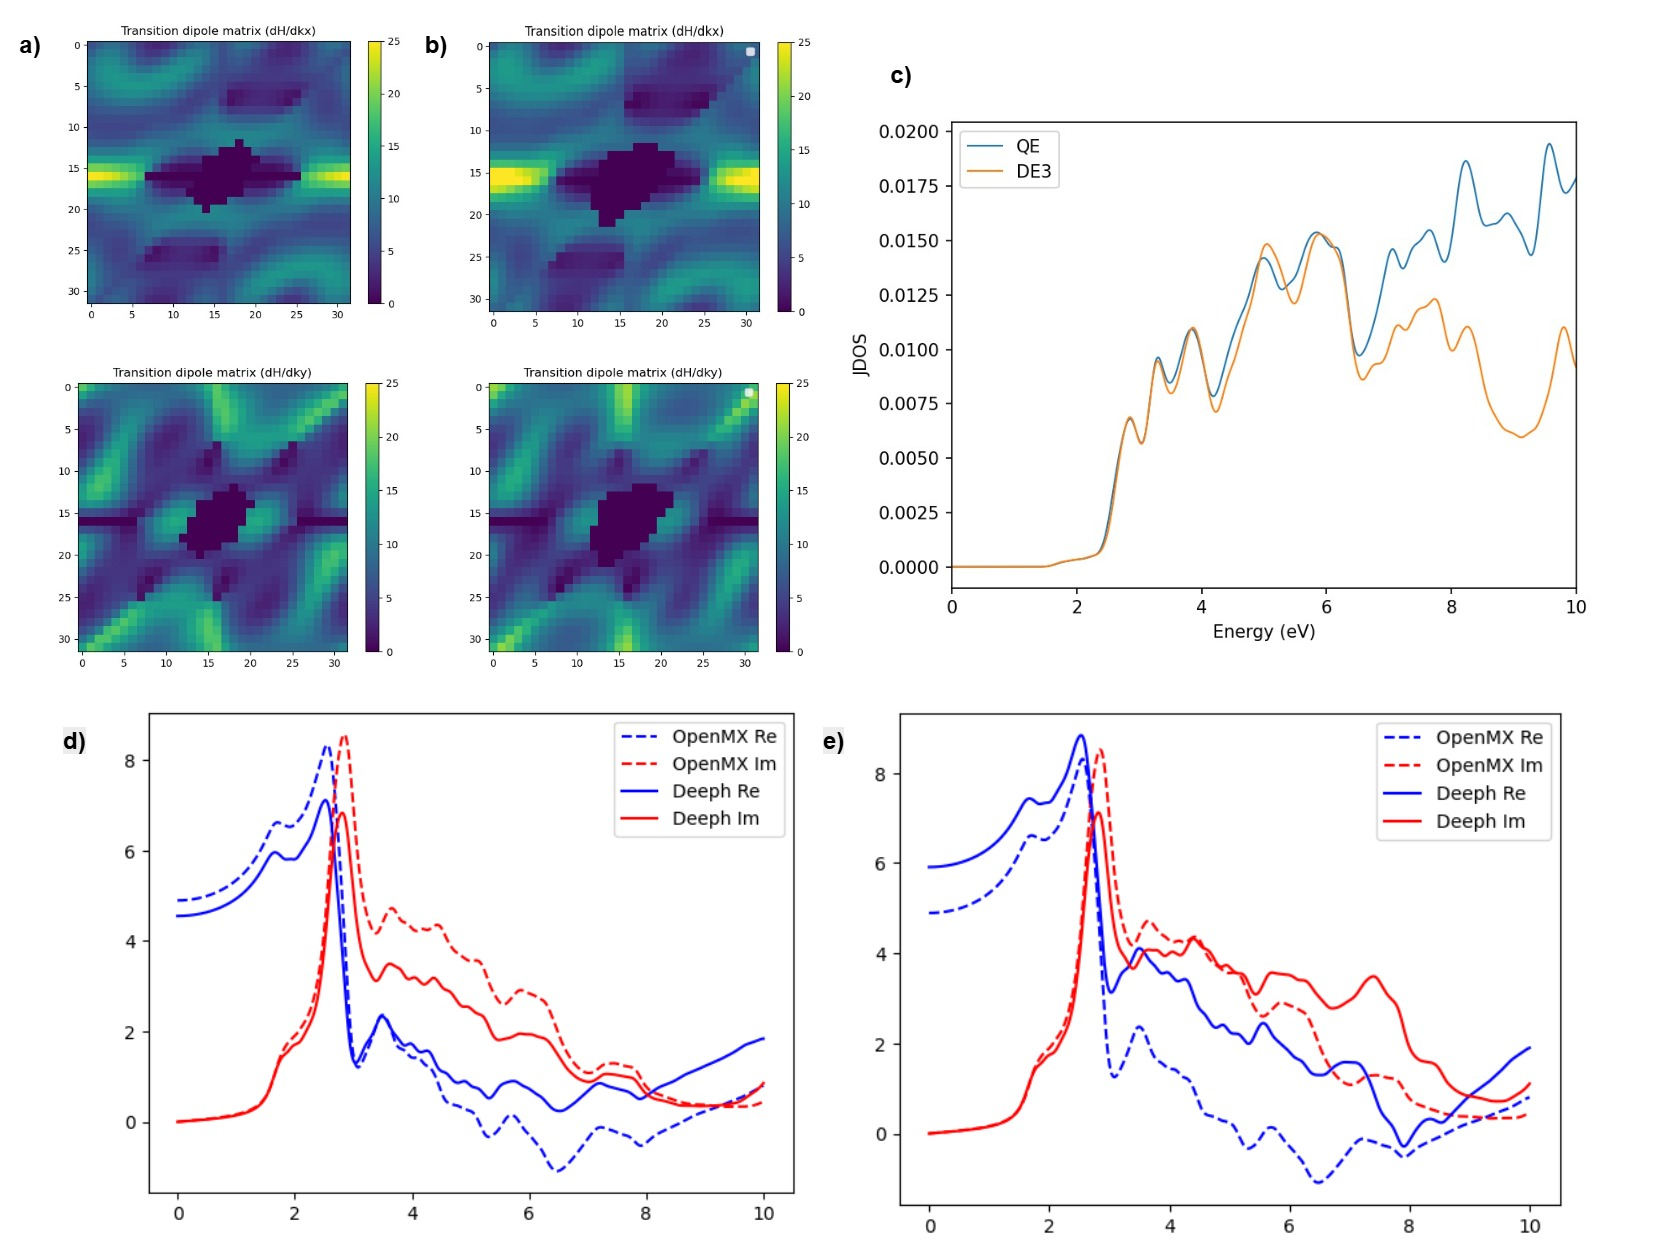
\includegraphics[height=10cm]{./img/optical_results.jpg}			
	\caption{}		%Make your caption descriptive
	\label{fig:optical}			%so you can reference to the figure elsewhere using \ref{}
\end{figure}

\red{(mention typical method for optical--wannierize, tight binding)--if not in lit review already}

Several optical effects were computed from the DeepH Hamiltonian, as shown in Figure \ref{fig:optical}. The accuracy in the transition dipole matrix indicates that the method used to orthogonalize and differentiate the Hamiltonian is reliable. The joint density of states (JDOS) and dielectric function, while inexact, capture the positions of peaks and their rough amplitudes. As optical functions computed solely from atomic structure are notoriously tricky, the low error can be considered extremely encouraging. 

The JDOS is accurate up to approximately 7eV; this can be attributed to the fact that Quantum ESPRESSO utilises a plane wave basis set, which--unlike the localised atomic orbitals used by OpenMX and DeepH--captures vacuum states above the Fermi level. As shown in \ref{figure}, the bandstructures computed in OpenMX and Quantum ESPRESSO diverge wildly above 7eV. \red{Fortunately, 7eV in photon-ese corresponds to UV light. Which is kind of important actually so this isn't very fortunate after all. Do proper discussion on whether this is good/ bad/ worrying/ important}

Notably, the DFT reference results for each optical effect were generated using different softwares; nonetheless, DeepH achieved encouraging similarities with all three.

\red{compare the calculation speed to wannier etc}

\section{Some remarks on training}

\red{(Not sure if I should have it here or on methods. Probably methods but I think I wanted to include Hamiltonian error heatmaps)}


\chapter{Conclusions}
\begin{itemize}
    \item results fairly good near Fermi level
    \item bad for: higher conduction bands (basis set dependent)
    \item k-space dependence: 
    \item disturbing results for strain
    \item note ease and speed of generating new training sets -- incentive for data-driven methods (gap between electronic structure methods and code for smaller vs very large systems is wide)
    
\end{itemize}



\small
\printbibliography			%inserts the bibliography, remember to specify your bib file in the preamble!
\end{document}